\documentclass[10pt,pdf,hyperref={unicode}]{beamer}

\usepackage[normalem]{ulem}
\usepackage{qrcode}
\usepackage{array}
\usepackage[T2A]{fontenc}
\usepackage[utf8]{inputenc}
\usepackage{colortbl}
\usepackage{minted}
\usepackage{listings}
\usepackage{tcolorbox}

\setbeamertemplate{navigation symbols}{}

\usetheme{default}

\usepackage{array}
\newcolumntype{L}[1]{>{\raggedright\let\newline\\\arraybackslash\hspace{0pt}}m{#1}}
\newcolumntype{C}[1]{>{\centering\let\newline\\\arraybackslash\hspace{0pt}}m{#1}}
\newcolumntype{R}[1]{>{\raggedleft\let\newline\\\arraybackslash\hspace{0pt}}m{#1}}

\definecolor{shadecolor}{RGB}{210,210,210}
\newcommand{\asm}[1]{\colorbox{shadecolor}{#1}}

\newcommand{\qrlinkframe}[2]{\begin{frame}{#1}
\center\qrcode[hyperlink,height=75px]{#2}
\end{frame}}

\title{Семинар 8: Intel x86 assembly. Часть 2}
\date{14 января, 2020}


\begin{document}

\begin{frame}
  \titlepage
\end{frame}

\begin{frame}{Работа с памятью}
        AT\&T:\\
        \begin{center}\lstinline{disp(base, index, scale)}\end{center}
        Intel:\\
        \begin{center}\lstinline{[base + index*scale + disp]}\end{center}

    \begin{itemize}
        \item base — базовый регистр, index — <<индексирующий>>
        \item scale $\in \{1, 2, 4, 8\}$
        \item disp (displacement) — signed 32 bit
        \item Результирующий адрес: \lstinline{base + index*scale + disp}
    \end{itemize}
\end{frame}

\begin{frame}[fragile]
\frametitle{Работа с памятью: примеры}
    Intel:
    \begin{minted}{nasm}
        mov rax, [rax]
        mov rax, [rax + rcx]
        mov rax, [rax + 8]
        mov rax, [rax + 4*rcx]
        mov rax, [rax + 2*rcx + 0x10]
    \end{minted}

    AT\&T:
    \begin{minted}{gas}
        mov (%rax), %rax
        mov (%rax, %rcx), %rax
        mov 8(%rax), %rax
        mov (%rax, %rcx, 4), %rax
        mov 0x10(%rax, %rcx, 2), %rax
    \end{minted}
\end{frame}

\begin{frame}{Подпрограммы}
    \begin{itemize}
        \item Уже видели \asm{call} — вызов <<подпрограммы>>
        \item Программа с точки зрения ассемблера — последовательность инструкций
        \item Подпрограмма — это последовательность инструкций с прикреплённым к нему контекстом или \emph{stack frame}
        \item \asm{call arg} запоминает текущий адрес — \emph{адрес возврата} и совершает безусловный прыжок по адресу в аргументе
        \item \asm{ret} забирает запомненный адрес возврата и передаёт управление обратно
    \end{itemize}
\end{frame}

\begin{frame}{Подпрограммы: аргументы}
    \begin{itemize}
        \item Как передавать аргументы?
        \item Calling conventions или ABI — \emph{application binary interface}
        \item Будем изучать System V AMD64 ABI
    \end{itemize}
\end{frame}

\begin{frame}{x86 stack and calling conventions}
\begin{itemize}
    \item Состоит из последовательных фреймов, образующих \emph{stack trace}
    \item Хранит локальные переменные и адрес возврата
    \item Растёт противоположно росту адресов: больший адрес соответствует <<дну>> стека
    \item \textbf{esp} указывает на первый свободный байт стека
    \item \textbf{ebp} указывает на начало текущего фрейма
    \item Всё, что ниже \textbf{ebp} — локальные переменные
    \item Выше расположены: начало предыдущего фрейма (предыдущий \textbf{ebp}),  адрес возврата и аргументы
\end{itemize}
\end{frame}

\begin{frame}{Картинка для понимания}
\center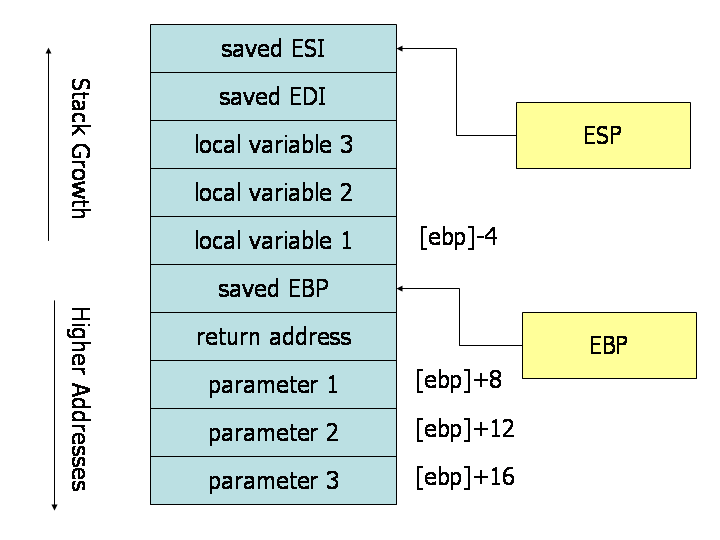
\includegraphics[scale=0.3]{stack.png}
\end{frame}

\begin{frame}{Register preserving}
\begin{itemize}
    \item Что делать с регистрами?
    \item Давайте договоримся какие нужно сохранять, а какие — нет
    \item Caller-saved registers: \textbf{eax}, \textbf{ecx}, \textbf{edx}
    \item Callee-saved registers: \textbf{ebx}, \textbf{esi}, \textbf{edi}, \textbf{ebp}, \textbf{esp}
    \item \textbf{eax} содержит возвращаемое значение (если оно целочисленное)
\end{itemize}
\end{frame}

\begin{frame}{Передача аргументов под x86}
\begin{itemize}
    \item Кладутся на стек в \textbf{обратном} порядке — последний пушится первым
    \item Первый аргумент лежит в \textbf{ebp + 8} (пропускается старый ebp и адрес возврата)
    \item Заполняются и очищаются вызывающей стороной, callee не должен их изменять
\end{itemize}
\end{frame}

\begin{frame}{x86-64 calling conventions}
\begin{itemize}
    \item Кладутся в регистры \textbf{обратном} порядке — последний пушится первым
    \item Порядок аргументов: \textbf{rdi}, \textbf{rsi}, \textbf{rdx}, \textbf{rcx}, \textbf{r8}, \textbf{r9}
    \item Caller-saved: \textbf{rax}, \textbf{rdi}, \textbf{rsi}, \textbf{rdx}, \textbf{rcx}, \textbf{r8}, \textbf{r9}, \textbf{r10}, \textbf{r11}
    \item Callee-saved: \textbf{rbx}, \textbf{rsp}, \textbf{rbp}, \textbf{r12}, \textbf{r13}, \textbf{r14}, \textbf{r15}
\end{itemize}
\end{frame}

\begin{frame}[fragile]
\frametitle{Пролог и эпилог функции}
\begin{center}
    \begin{minted}{gas}
                # Пролог
    push %ebp          # Запоминаем предыдущий фрейм
    mov %esp, %ebp     # Запоминаем начало текущего фрейма
    push %ebx          # Сохраняем callee-saved регистры
    push %edi
    # ...
    sub $16, %esp      # Выделяем место на стеке

            # ... ваша функция ...

                # Эпилог
    add $16, %esp      # Освобождаем место на стеке
    # ...
    pop %edi           # Восстанавливаем регистры
    pop %ebx
    mov %ebp, %esp     # Восстанавливаем текущий фрейм
    pop %ebp           # Восстанавливаем предыдущий фрейм
    ret                # Возвращаемся из функции
    \end{minted}
\end{center}
\end{frame}

\begin{frame}{Выравнивание стека}
\begin{itemize}
    \item Необходимо, чтобы не использовать лишних and'ов
    \item В современных ABI — 16 байт
    \item Под x86 гарантируется, что первый аргумент выровнен по 16ти байтам
    \item Выравнивать нужно \emph{перед} \asm{call} и \emph{перед} заполнением аргументов
    \item Если не выровнять стек, то, скорее всего, получите segfault!
\end{itemize}
\end{frame}

\qrlinkframe{Про calling conventions}{https://wiki.osdev.org/Calling\_Conventions}

\begin{frame}
\center\Huge{Gracias!}
\end{frame}


\end{document}
